% !TEX encoding = UTF-8 Unicode
\chapter{Prova pratica}%tante immaginine

\section{Installazione}
Per installare il progetto \'e necessario che nel sistema siano installati \emph{python, pip} e \emph{git}. Pip è uno strumento comodo per installare pacchetti per python, mentre Git è un software di controllo versioni e di gestione del codice. Tramite Git è possibile creare dei repository che permettono di effettuare degli \emph{snapshot}, ossia delle \emph{fotografie} degli stati del progetto ed annullare modifiche se necessario, aggiungere nuove features ed inserirle nel progetto solo quando complete e funzionanti. Inoltre è comodo in caso di lavoro con altre persone, perché fornisce strumenti per unire il proprio lavoro con quello degli altri.

Con il comando seguente da eseguire sul terminale si effettua una copia nel proprio computer del repository contenente il progetto:

\begin{lstlisting}[language=c]
$ git clone https://github.com/andxet/piedmont-heritage.git
\end{lstlisting}

In questo modo il progetto sarà scaricato sul computer. Mongo deve essere avviato, basterà eseguire il seguente comando nella cartella dove scaricato e decompresso, che avvierà il demone che resterà in ascolto di connessioni:

\begin{lstlisting}[language=c]
$ mongo/bin/mongod
\end{lstlisting} 

Ora si può procedere all'installazione vera e propria.
\begin{lstlisting}[language=c]
$ cd piedmont-heritage
$ python setup.py develop
$ gearbox setup-app
\end{lstlisting} 

Questa sequenza di comandi si occupa di installare le dipendenze del progetto, tra cui Turbogears, inizializzare il progetto eseguendo la funzione di bootstrap, la quale carica sul database tutti i locali.

Infine si deve avviare il server http:
\begin{lstlisting}[language=c]
$ gearbox serve
\end{lstlisting} 

Questo comando crea un server attraverso gli strumenti di turbogears.
Non è consigliato utilizzare questa configurazione per la distribuzione del progetto perché è tarata per un utilizzo in caso di debug, perché non molto sicuro e per la presenza di messaggi di log.

Aprendo il browser all'indirizzo
\begin{lstlisting}
localhost:8080
\end{lstlisting} sarà possibile visualizzare il sito. Sarà necessaria una connessione ad internet anche se il sito è in locale, perché le mappe non sono comprese nel progetto e vengono scaricate dal sito opportuno al momento della visualizzazione.

\section{Esempio di sessione}
La pagina è divisa in sezioni: prima la mappa dei locali, poi un grafico che mostra le categorie, uno che mostra il resoconto dell'età dei locali, ed un resoconto degli oggetti storici. Il nostro interesse si focalizzerà sulla mappa, che apparirà inizialmente come nella figura \ref{fig:ini}.
La richiesta che riceve il server non contiene parametri, siccome l'url è quello mostrato precedentemente, quindi viene inviata la pagina html. Inizialmente la pagina non contiene la mappa ma un tag \texttt{div} che verrà riempito con l'oggetto mappa. Questa operazione è eseguita dalla funzione \texttt{drawMap()} richiamata a fondo pagina: gli elementi come il canvas contenente la mappa, i pulsanti di zoom e la mappa stessa vengono quindi aggiunti tramite codice, ed i dati da visualizzare con richieste asincrone dalla pagina al server. Il processo di creazione della mappa prevede anche il caricamento di default di tutti i comuni, i tipi ed i marker dei locali, che verranno ottenuti ognuno con richiesta diversa (Fig. \ref{fig:tipo} e \ref{fig:comuni}).

\begin{figure}[ht!]
	\caption{Aspetto della mappa all'apertura della pagina.}
	\label{fig:ini}
	\centering
		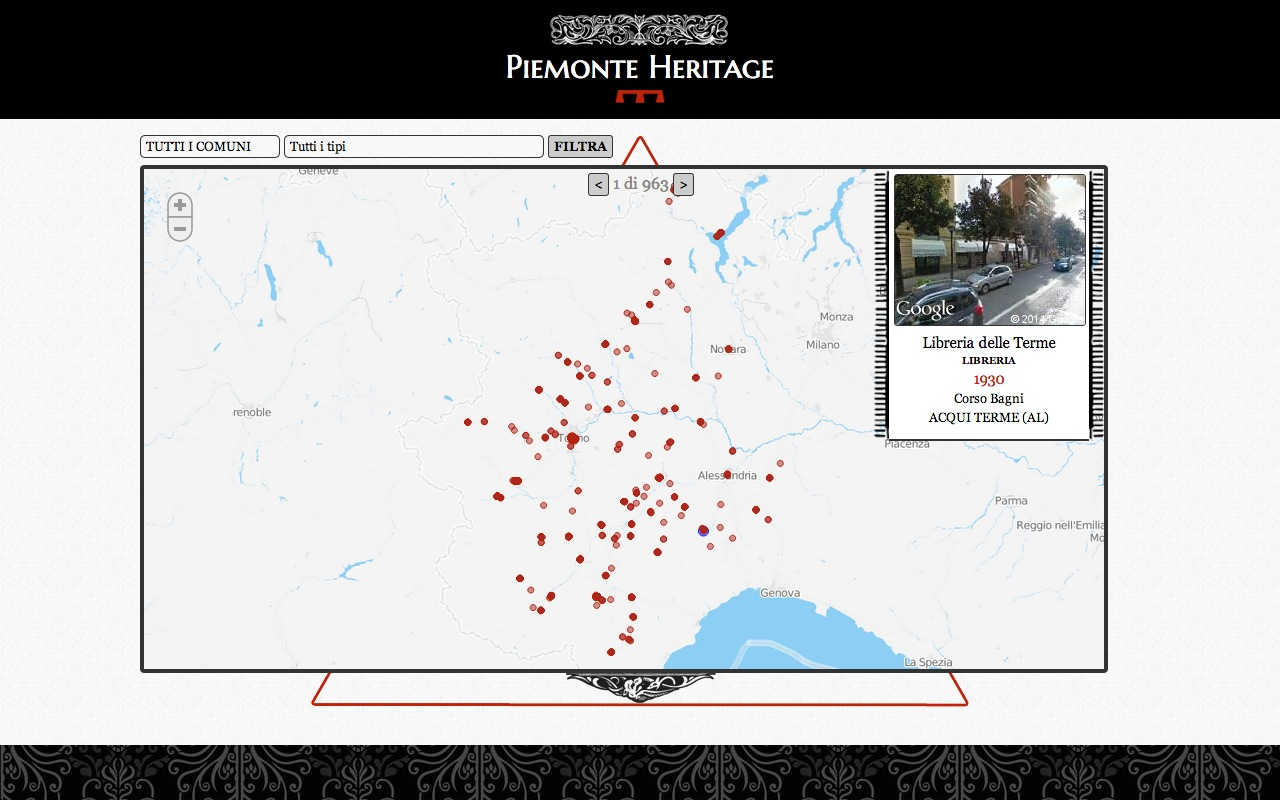
\includegraphics[width=\textwidth]{img/s1.jpg}
\end{figure}

I comuni ed i tipi sono aggiunti all'interno del relativo \texttt{select} tramite codice, creando il relativo tag \texttt{option}.

\begin{figure}[ht!]
	\caption{Elenco di tutte le tipologie disponibili}
	\label{fig:tipo}
	\centering
		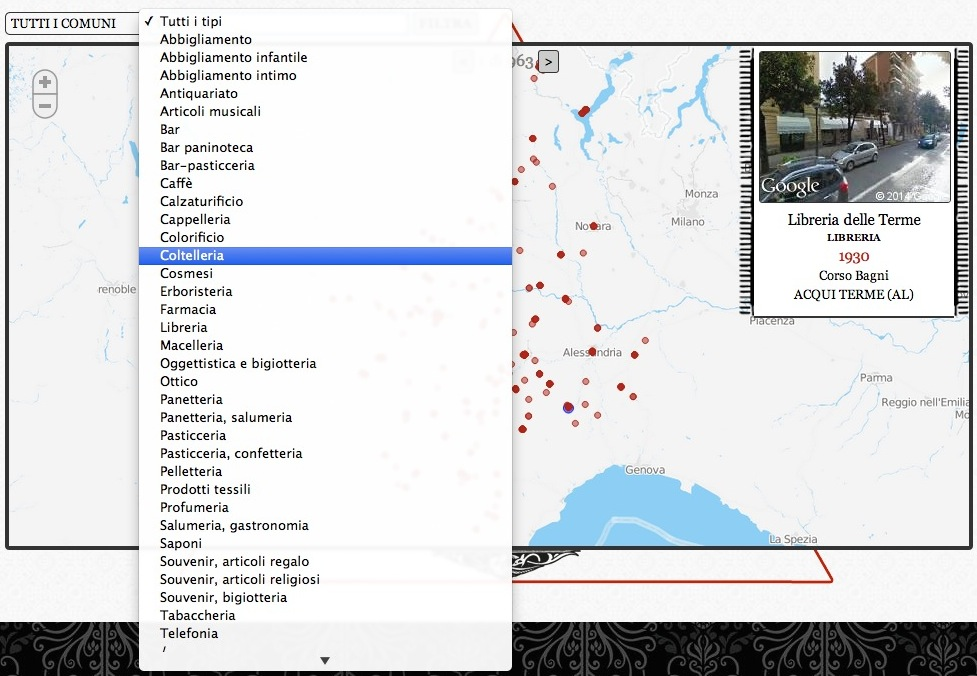
\includegraphics[width=\textwidth]{img/s2.jpg}
\end{figure}

Se un comune viene selezionato, si visualizzeranno nell'altro menu a tendina solo i tipi presenti in quel comune. Al click il client invia una richiesta al server con il comune come parametro, e riceve l'elenco di tipi, il menu a tendina viene prima svuotato e poi popolato dei risultati ricevuti.

\begin{figure}[ht!]
	\caption{Selezione del comune}
	\label{fig:comuni}
	\centering
		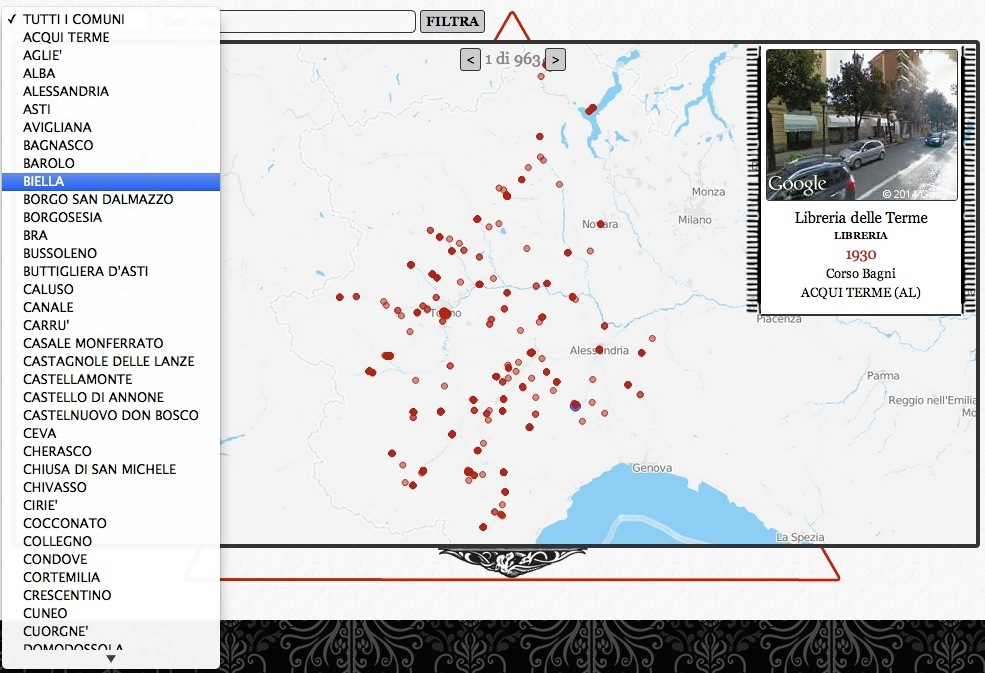
\includegraphics[width=\textwidth]{img/s3.jpg}
\end{figure}

\begin{figure}[ht!]
	\caption{Le tipologie mostrate sono solo quelle presenti nel comune selezionato}
	\centering
		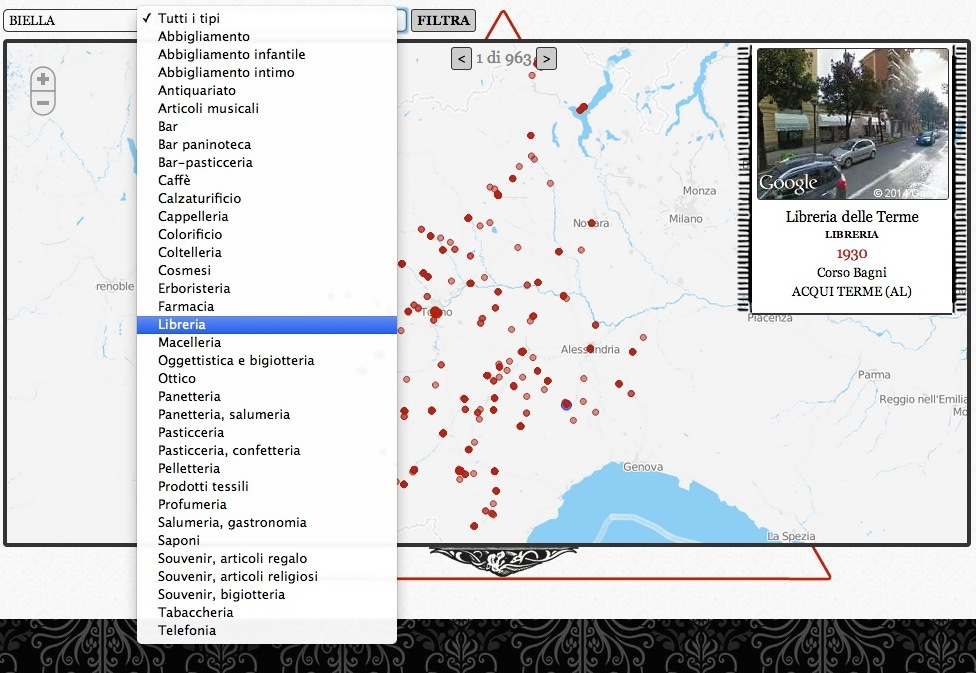
\includegraphics[width=\textwidth]{img/s4.jpg}
\end{figure}

Premendo filtra, il client effettua una richiesta al server inviando il comune ed il tipo come parametri. Le voci "Tutti i comuni" e "Tutti i tipi" valgono come valori nulli, indicano che non sono state espresse preferenze e non è necessario effettuare selezioni in base a quel campo. Il server restituisce una lista contenente le coordinate di tutti i punti e l'id del locale che rappresentano. Vengono quindi mostrati i marker sulla mappa e viene selezionato il primo, ossia viene effettuata una chiamata a \texttt{select()}, che diverrà blu e più grande, ed i dati verranno richiesti al server e mostrati nello specchietto in alto a destra. La mappa mostra solamente i punti filtrati ed adatta lo zoom in modo da mostrarli tutti .

\begin{figure}[ht!]
	\caption{Locali storici di Biella}
	\centering
		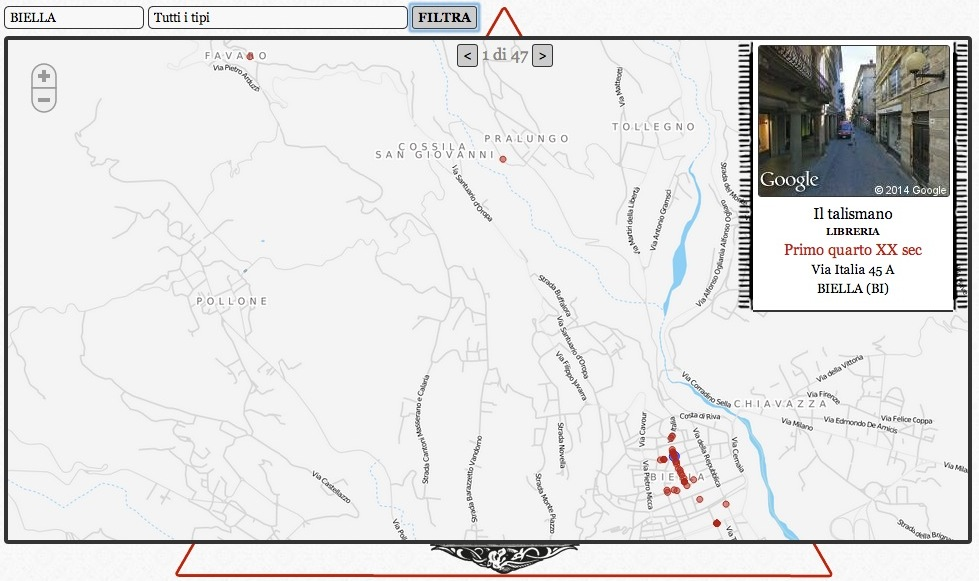
\includegraphics[width=\textwidth]{img/s5.jpg}
\end{figure}

I pulsanti di navigazione in alto al centro, richiamano rispettivamente le funzioni \texttt{prev()} e \texttt{next()}, che fanno retrocedere o proseguire l'iteratore della lista dei locali.

\begin{figure}[ht!]
	\caption{Premendo i pulsanti di navigazione viene selezionato il locale successivo, cambiandone l'indicatore da rosso a blu e centrandolo sulla mappa. I relativi dati inoltre vengono mostrati in alto a destra.}
	\centering
		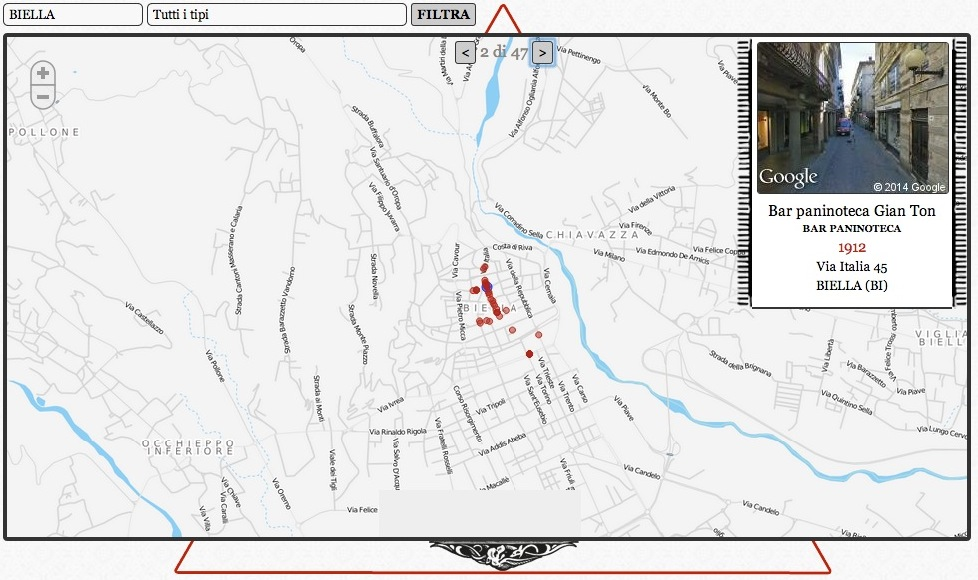
\includegraphics[width=\textwidth]{img/s6.jpg}
\end{figure}

Nel caso della figura \ref{fig:biella}, si sceglie di visualizzare i due bar di Biella presenti nel dataset. Il procedimento è uguale a quello descritto precedentemente, in questo caso si effettua la ricerca dei locali con comune="Biella" e tipo="Bar".

\begin{figure}[ht!]
	\caption{Selezionando una categoria e poi filtra, vengono mostrati solo i relativi punti.}
	\label{fig:biella}
	\centering
		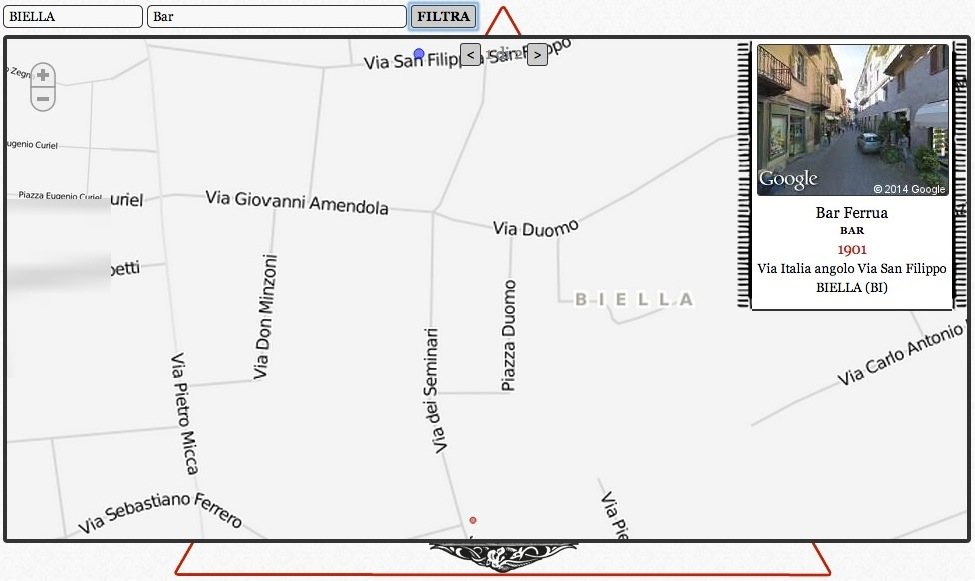
\includegraphics[width=\textwidth]{img/s8.jpg}
\end{figure}

Nel caso della fig. \ref{fig:solotipi} i criteri di ricerca sono solamente quelli per il tipo: tipo="Drogheria, salumeria, pizzicherie e simili".

\begin{figure}[ht!]
	\caption{Se lo si desidera, si pu\`o visualizzare tutti i locali dello stesso tipo in tutti i comuni.}
	\label{fig:solotipi}
	\centering
		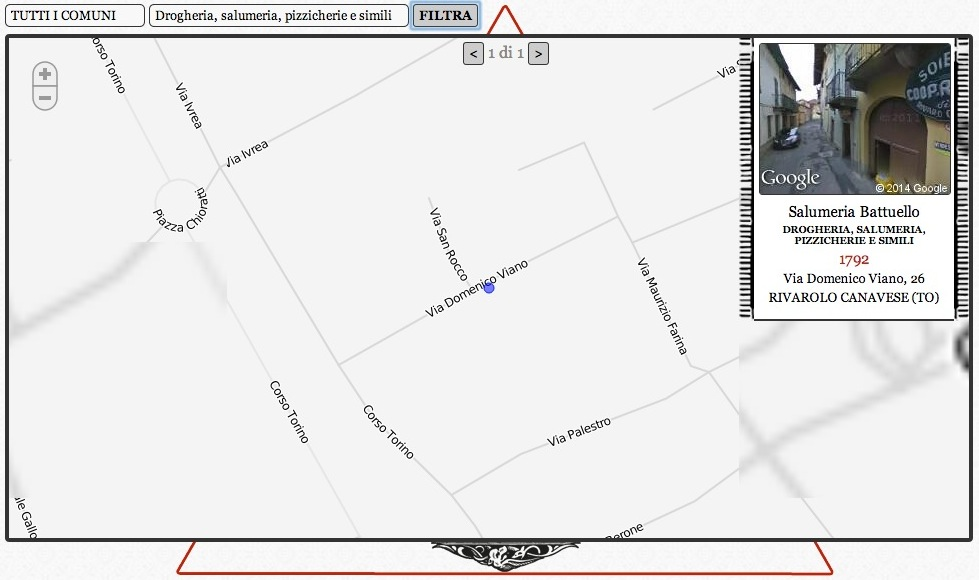
\includegraphics[width=\textwidth]{img/s9.jpg}
\end{figure}

Come descritto nei precedenti capitoli, la natura del dataset comporta la presenza di dati errati o non coerenti.

\begin{figure}[ht!]
	\caption{I record non contengono dati esatti: l'ubicazione memorizzata \`e nel comune di Torino, ma le coordinate sono inesatte.}
	\centering
		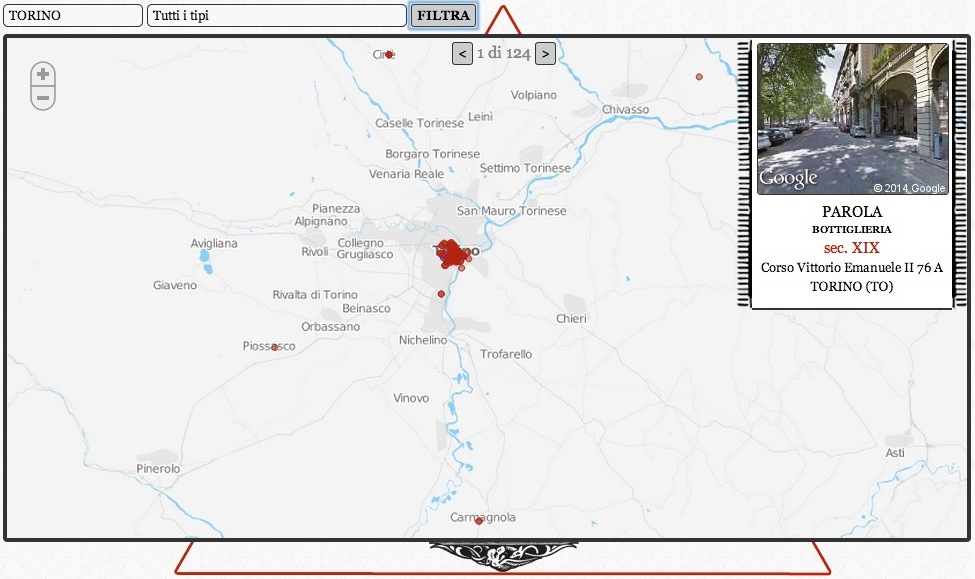
\includegraphics[width=\textwidth]{img/s11.jpg}
\end{figure}

La mappa è completamente interattiva: oltre alla possibilità di filtrare i risultati, è possibile scorrere la mappa cliccando su di essa e facendo scorrere il mouse, aumentare o diminuire lo zoom con la rotellina del mouse o con i pulsanti in alto a sinistra. Cliccando sui punti essi verranno selezionati, ed i dettagli del locale che rappresentano mostrati nello specchietto in alto a destra.

\begin{figure}[ht!]
	\caption{Cliccando su un puntino esso verr\`a selezionato.}
	\centering
		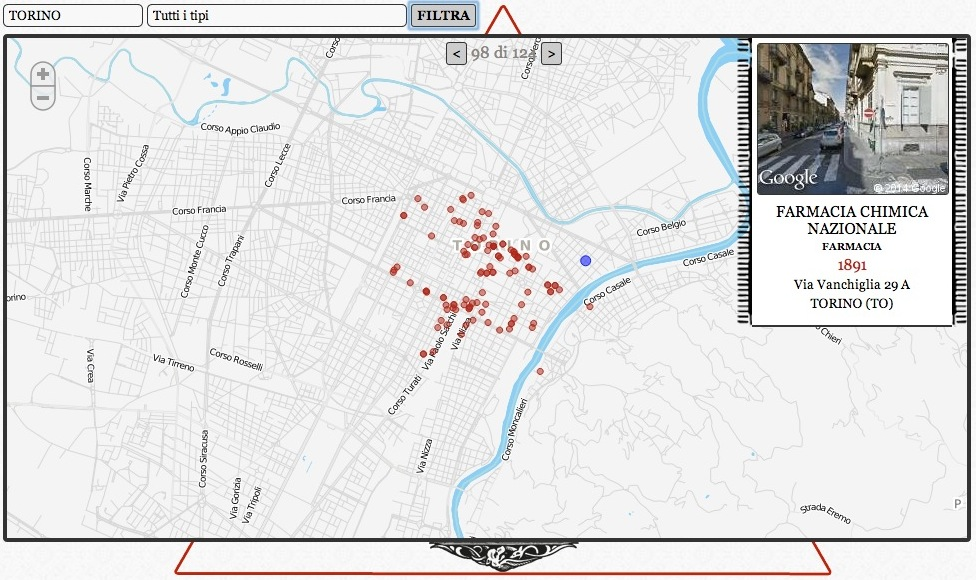
\includegraphics[width=\textwidth]{img/s13.jpg}
\end{figure}